\documentclass{beamer}[10pt, usepdftitle=false, handout]

\beamertemplatenavigationsymbolsempty

\usepackage[T1]{fontenc}
\usepackage[]{algorithm2e}
\usepackage{multimedia}
\usepackage{gensymb}
\usepackage{textcomp}
\usepackage{color}
\usepackage{background}
%\backgroundsetup{
%    placement=center,
%    scale=1,
%    contents={The author of this course is PAUL BLONDEL},
%    opacity=0.7
%}
%\setbeamertemplate{background}{\BgMaterial}
%\usepackage[font=small,labelfont=bf]{caption} 

\usetheme{Boadilla}

\title{Data Structure 3}
\author[]{Paul Blondel}
\institute[]{CNAM}
\date[]{September 1st, 2018}

\usepackage[style=british]{csquotes}


\def\signed #1{{\leavevmode\unskip\nobreak\hfil\penalty50\hskip1em
  \hbox{}\nobreak\hfill #1%
  \parfillskip=0pt \finalhyphendemerits=0 \endgraf}}

\newsavebox\mybox
\newenvironment{aquote}[1]
  {\savebox\mybox{#1}\begin{quote}\openautoquote\hspace*{-.7ex}}
  {\unskip\closeautoquote\vspace*{1mm}\signed{\usebox\mybox}\end{quote}}


%\setbeamertemplate{headline}
%{
%  \leavevmode%
%  \hbox{%
%  \begin{beamercolorbox}[wd=1.0\paperwidth,ht=2.25ex,dp=1ex,center]{author in head/foot}%
%   \textcolor{green}{- This course has been made by Paul Blondel -} \usebeamerfont{author in head/foot}\insertsubsection
%  \end{beamercolorbox}}%
%  \vskip0pt%
%}


\setbeamertemplate{footline}
{
  \leavevmode%
  \hbox{%
  \begin{beamercolorbox}[wd=.5\paperwidth,ht=2.25ex,dp=1ex,center]{author in head/foot}%
    \usebeamerfont{author in head/foot}\insertsection
  \end{beamercolorbox}%
  \begin{beamercolorbox}[wd=.5\paperwidth,ht=2.25ex,dp=1ex,center]{title in head/foot}%
    \usebeamerfont{title in head/foot} \inserttitle \hspace*{2em}  \insertframenumber{} / \inserttotalframenumber\hspace*{2ex} 
  \end{beamercolorbox}}%
  \vskip0pt%
}

\AtBeginSection[]
{
   \begin{frame}
    \tableofcontents[ 
    currentsection] 
   \end{frame}
}
\SetKw{KwBy}{by}

\begin{document}
	{
	\setbeamertemplate{footline}{
  	\leavevmode%
  	\hbox{%
  	\begin{beamercolorbox}[wd=.5\paperwidth,ht=2.25ex,dp=1ex,center]{author in head/foot}%
  	\end{beamercolorbox}%
  	\begin{beamercolorbox}[wd=.5\paperwidth,ht=2.25ex,dp=1ex,center]{title in head/foot}%
  	\end{beamercolorbox}}%
  	\vskip0pt%	
	} 
	\begin{frame}
	\titlepage
	\end{frame}

	\begin{frame}
	
	\begin{aquote}{Linus Torvalds}
	I will, in fact, claim that the difference between a bad programmer and a good one is whether he 
	considers his code or his data structures more important. Bad programmers worry about the code. Good programmers worry about data structures and their relationships.	
	\end{aquote}	
	
	\end{frame}


	\begin{frame}
		\tableofcontents
	\end{frame}
	}

	\addtocounter{framenumber}{-3}

	\section{Sorting algorithms}	

    \begin{frame}[label=(first)]
		
	\begin{block}{Recall}
	Sorted arrays are \textbf{more efficient in search}	
	\end{block}
	
	\vspace*{1em}	
	
	Besides, many algorithms need sorted arrays to work:
	
	\vspace*{1em}
	
	\begin{itemize}
	\item {Dijkstra's algorithm (finding shortest path)}
	\item {Prim's algorithm (finding minimum spanning tree)}
	\item {Kurskal's algorithm (finding minimum spanning tree)}
	\item {many more...}
	\end{itemize}		
	
    \end{frame}
	
	\begin{frame}

	We will study the following sorting approaches:
	
	\vspace*{1em}	
	
	\begin{itemize}
	\item{Selection sort}
	\item {Insertion sort}
	\item {Quick sort}
	\item {Heap sort}
	\item {Bubble sort}
	\end{itemize}
	
	\end{frame}

	\section {Selection sort}
	
	\begin{frame}
	
	\begin{block}{Principle}
	\textbf{Swap} the current value with the \textbf{smallest unsorted value} 
	\end{block}	
	
	\begin{columns}[c]
	\column{.55\textwidth} 
	\begin{center}    
    \scalebox{0.75} {
    %\begin{minipage}
    \begin{algorithm}[H]
    	i=0;j=0\;
		\While{$i < Array.length - 1$} {
			min=i\;
			j=i+1\;
			\While{j < Array.length} {
				\If{Array[j] < Array[min]} {
					min=j\;
				}
				j=j+1\;
			}
			temp=Array[i]\;
			Array[i]=Array[min]\;
			Array[min]=temp\;
			i=i+1\;
		}	 
 	%\caption{Sequential search through the array}
	\end{algorithm}	
	%\end{minipage}
	}
	\end{center}			
	
	\column{.45\textwidth}
	\begin{center}
	Complexities:
	
	comparisons = $O(N^2)$	
	
	swaps = $O(N)$
	
	\vspace*{1em}
	Example:
	\vspace*{1em}	
	
	step 0: \textbf{29}, 64, 73, 34, \textcolor{green}{20}
	
	step 1: \textit{20}, \textbf{64}, 73, 34, \textcolor{green}{29}
	
	step 2: \textit{20}, \textit{29}, \textbf{73}, \textcolor{green}{34}, 64
	
	step 3: \textit{20}, \textit{29}, \textit{34}, \textbf{73}, \textcolor{green}{64}
	
	step 4: \textit{20}, \textit{29}, \textit{34}, \textit{64}, \textit{73} 		
	
	\end{center}	
		
	\end{columns}
		
	\end{frame}	
	
	\section {Insertion sort}
	
	\begin{frame}
	\begin{block}{Principle}
	Move from \textbf{right to left} the unsorted value \textbf{to the best position}
	\end{block}	
	
	\begin{columns}[c]
	\column{.6\textwidth} 
	\begin{center}    
    \scalebox{0.75} {
    %\begin{minipage}
    \begin{algorithm}[H]
	i=1;j=0\;
	\While{$i < Array.length$} {
		val = Array[i]\;
		j=i\;
		
		\While{$j>0$ and $Array[j-1] > val$} {
			Array[j] = Array[j-1]\;
			j=j-1\;		
		} 
		Array[j] = val\;	
	}
 	%\caption{Sequential search through the array}
	\end{algorithm}	
	%\end{minipage}
	}
	\end{center}			
	
	\column{.4\textwidth}
	\begin{center}
%	Complexities:
%	
%	\begin{itemize}
%	\item {At best = $O(N)$, $O(1)$}
%	\item {Worst/Average = $O(N^2)$, $O(N)$}
%	\end{itemize}		
%	\vspace*{1em}
	Example:
	\vspace*{1em}	
	
	step 0: \textit{29}, \textbf{20}, 73, 34, 64

	step 1: \textit{20}, \textit{29}, \textbf{73}, 34, 64

	step 2: \textit{20}, \textit{29}, \textit{73}, \textbf{34}, 64

	step 3: \textit{20}, \textit{29}, \textit{34}, \textit{73}, \textbf{64}

	step 4: \textit{20}, \textit{29}, \textit{34}, \textit{64}, \textit{73}
		

	\end{center}	
		
	\end{columns}
			
	\vspace*{1em}
	Complexities: 
	
	\begin{itemize}
		\item {Best: $O(N)$ for comparisons, $O(1)$ for swaps}
		\item {Worst/Average: $O(N^2)$ for comparisons and swaps}
	\end{itemize}				
			
			
	\end{frame}	
	
	\section {Bubble sort}

	\begin{frame}
	
	\begin{block}{Principle}
	\textbf{Compare each value to the next and swap} if required (bubbling)
	\end{block}	
	
	\begin{columns}[c]
	\column{.6\textwidth} 
	\begin{center}    
    \scalebox{0.75} {
    %\begin{minipage}
    \begin{algorithm}[H]
	i=Array.length-1;j=0\;
	\While{i >= 0} {
		j=1\;
		\While{i <= i} {
			\If{Array[j-1] > Array[j]} {
				temp = Array[j-1]\;			
				Array[j-1] = Array[j]\;
				Array[j] = temp\;			
			}	
			j=j+1\;	
		}	
		i=i-1\;
	}	
	
 	%\caption{Sequential search through the array}
	\end{algorithm}	
	%\end{minipage}
	}
	\end{center}			
	
	\column{.4\textwidth}
	\begin{center}
	%Complexity = $O(N^2)$
	
	\vspace*{1em}
	Example:
	\vspace*{1em}	
	
	step 0: \textbf{7}, \textcolor{green}{5}, 2, 4, 3, 9
	
	step 1: \textit{5}, \textbf{7}, \textcolor{green}{2}, 4, 3, 9

	step 2: \textit{5}, \textit{2}, \textbf{7}, \textcolor{green}{4}, 3, 9

	step 3: \textit{5}, \textit{2}, \textit{4}, \textbf{7}, \textcolor{green}{3}, 9

	step 4: \textit{5}, \textit{2}, \textit{4}, \textit{3}, \textbf{7}, \textcolor{green}{9}

	step 5: \textit{5}, \textit{2}, \textit{4}, \textit{3}, \textit{7}, \textit{9}

	\end{center}	
		
	\end{columns}
	
	\vspace*{1em}
	Complexities:
	
	\begin{itemize}
	\item {Best: $O(N)$ for comparisons, $O(1)$ for swaps}
	\item {Worst/Average: $O(N^2)$ for comparisons, $O(N^2)$ for swaps}
	\end{itemize}			
	
	\end{frame}

	\section {Heap sort}
	\subsection{Principle}

	\begin{frame}
	
	\begin{block}{Principle}
	\begin{itemize}
	\item {The input array is \textbf{seen as a \textit{binary tree}} where: 
		\begin{itemize}
			\item {element i has children at index $2\times i$ and $2\times i+1$}
		\end{itemize}
	}
	\item {The binary tree is \textit{then} \textbf{transformed into a \textit{binary heap}}}
	\item {The \textbf{root node value is removed from the tree (it's sorted now)}\footnotemark}	
	\item {The new tree is \textbf{transformed back to a binary heap}, and so on}
	\end{itemize} 
	\end{block}

	\begin{center}
	
	\begin{figure}
		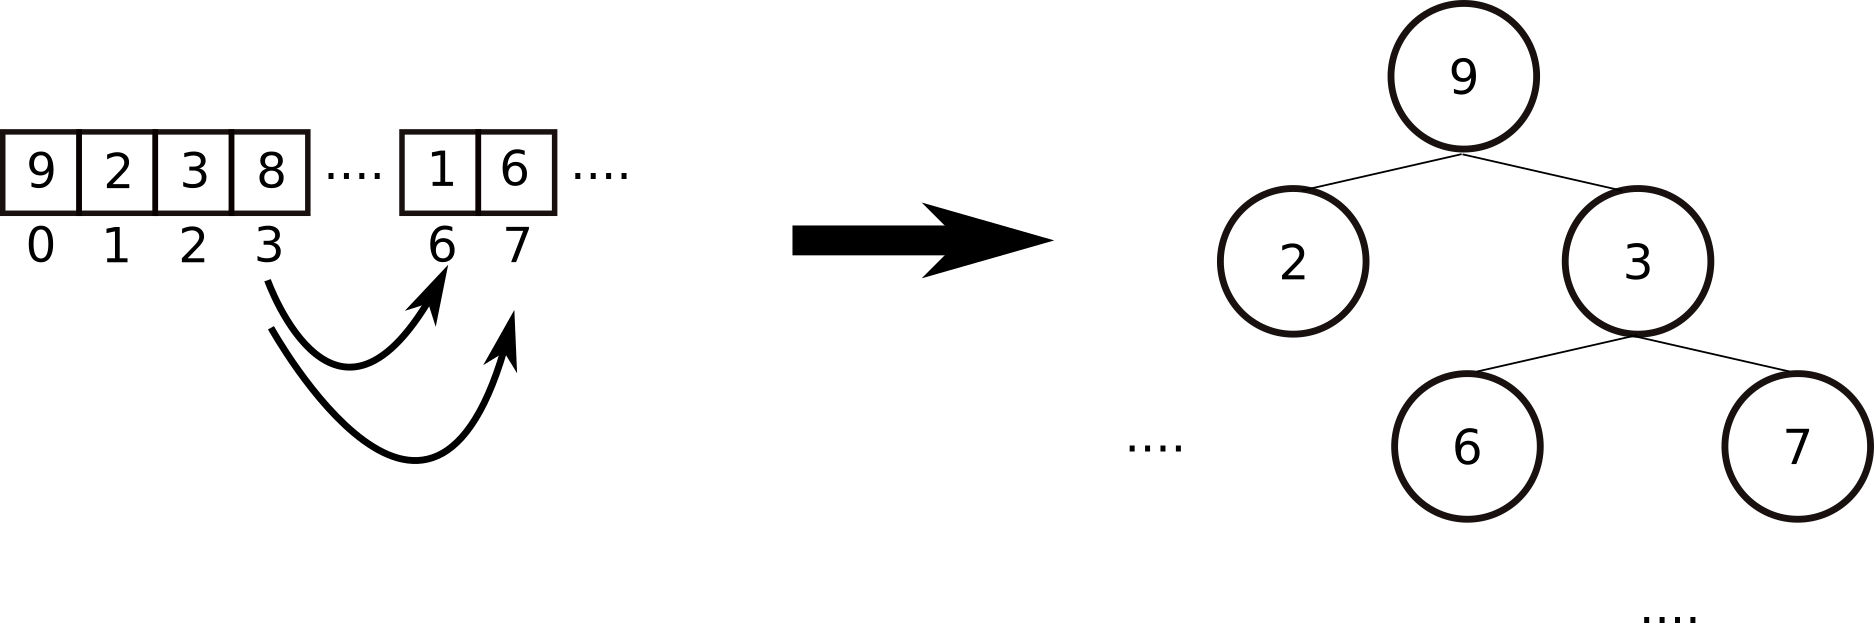
\includegraphics[scale=0.25]{images/array_as_binary_tree.png} 
     	%\vspace*{-0.5em}
		%\caption{Floating gate transistor cell}
	\end{figure}	
	\end{center}
		
	\footnotetext{The previous root node value is \textbf{not reinserted} in the tree.}		
		
	\end{frame}
		
	\begin{frame}
		
	A \textit{binary tree} is transformed into a \textit{(max) binary heap} if:
	
	\begin{itemize}
	\item {each node has a \textbf{value greater than those of its two children}}	
	\end{itemize}		
	
	Example:
	
	\begin{center}
	
	\begin{figure}
		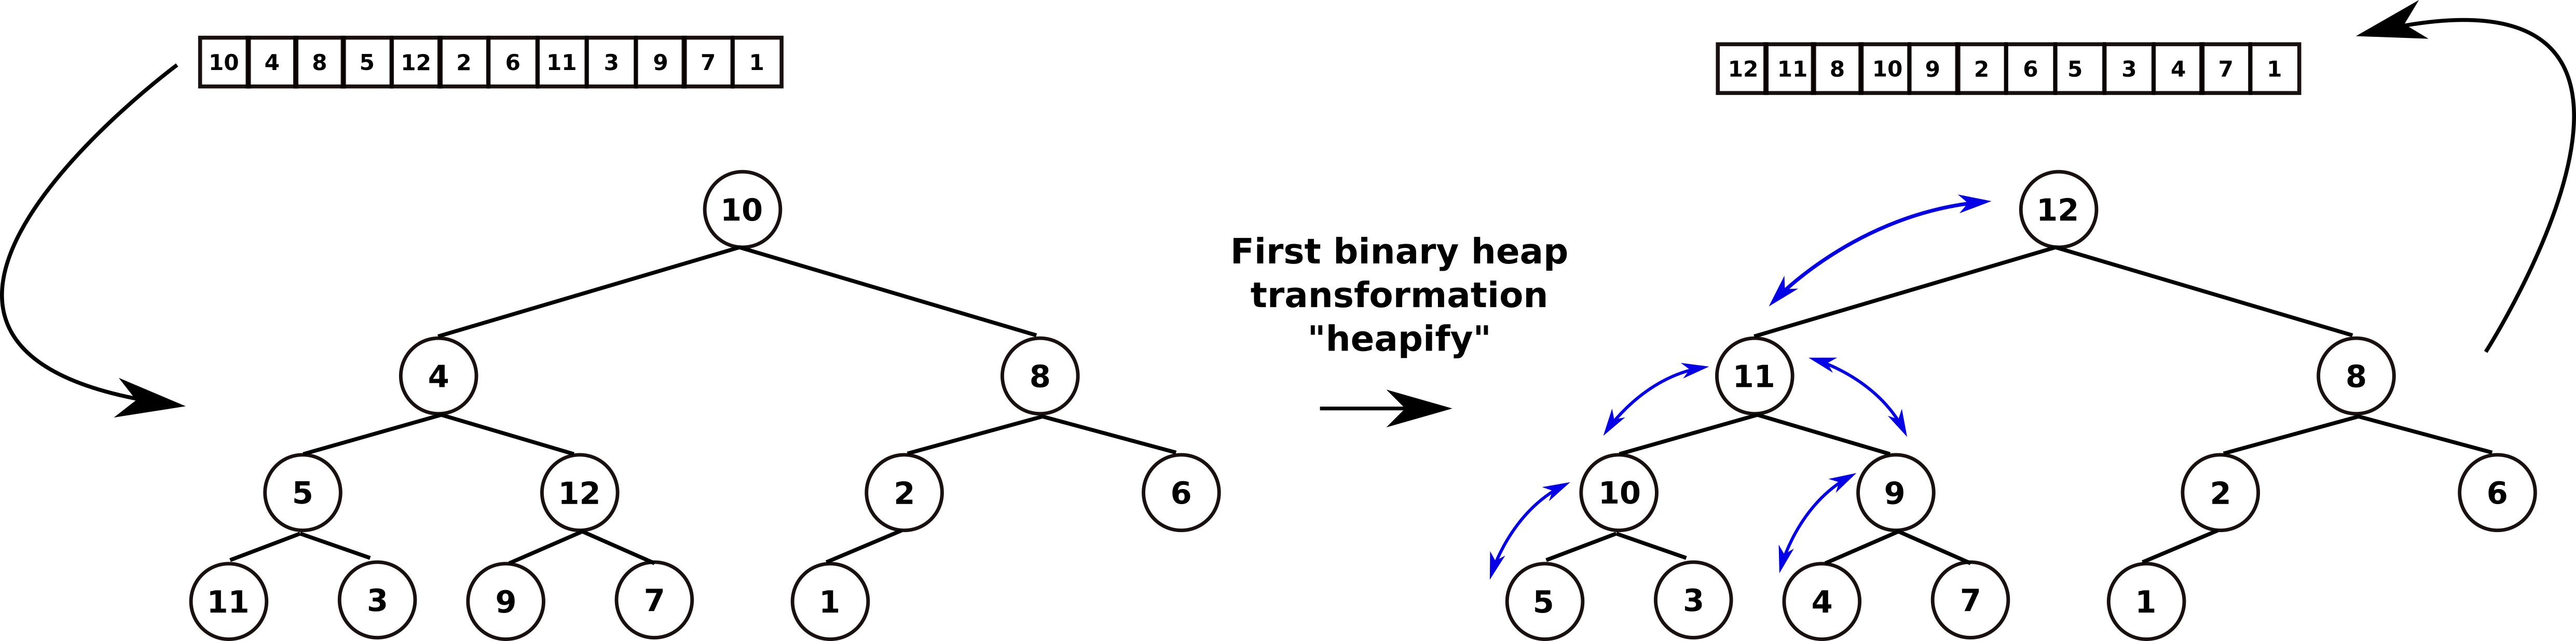
\includegraphics[scale=0.148]{images/heap_example_01.png} 
     	%\vspace*{-0.5em}
		%\caption{Floating gate transistor cell}
	\end{figure}	
	\end{center}
		
	\end{frame}	

	\begin{frame}
	
	\begin{center}	
	\begin{figure}
		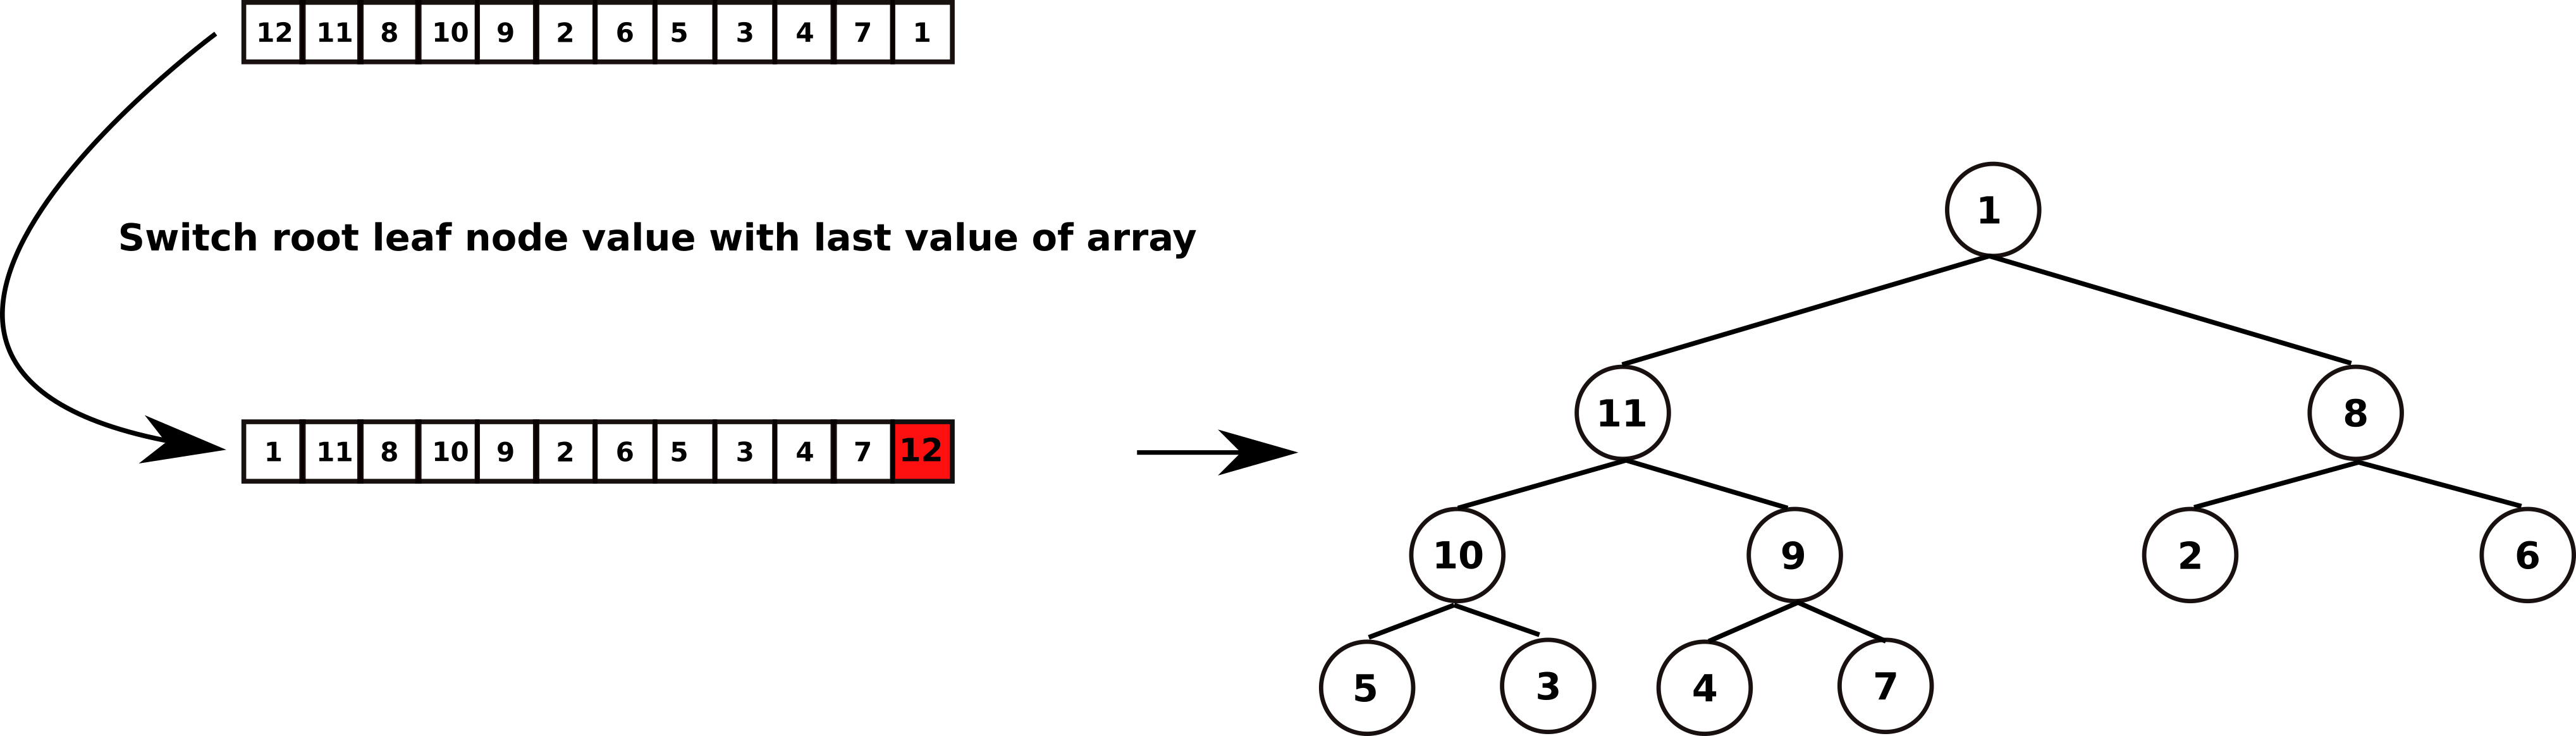
\includegraphics[scale=0.148]{images/heap_example_02.png} 
     	%\vspace*{-0.5em}
		%\caption{Floating gate transistor cell}
	\end{figure}	
	\end{center}
	
	\vspace*{1em}	
	
	\begin{center}	
	\begin{figure}
		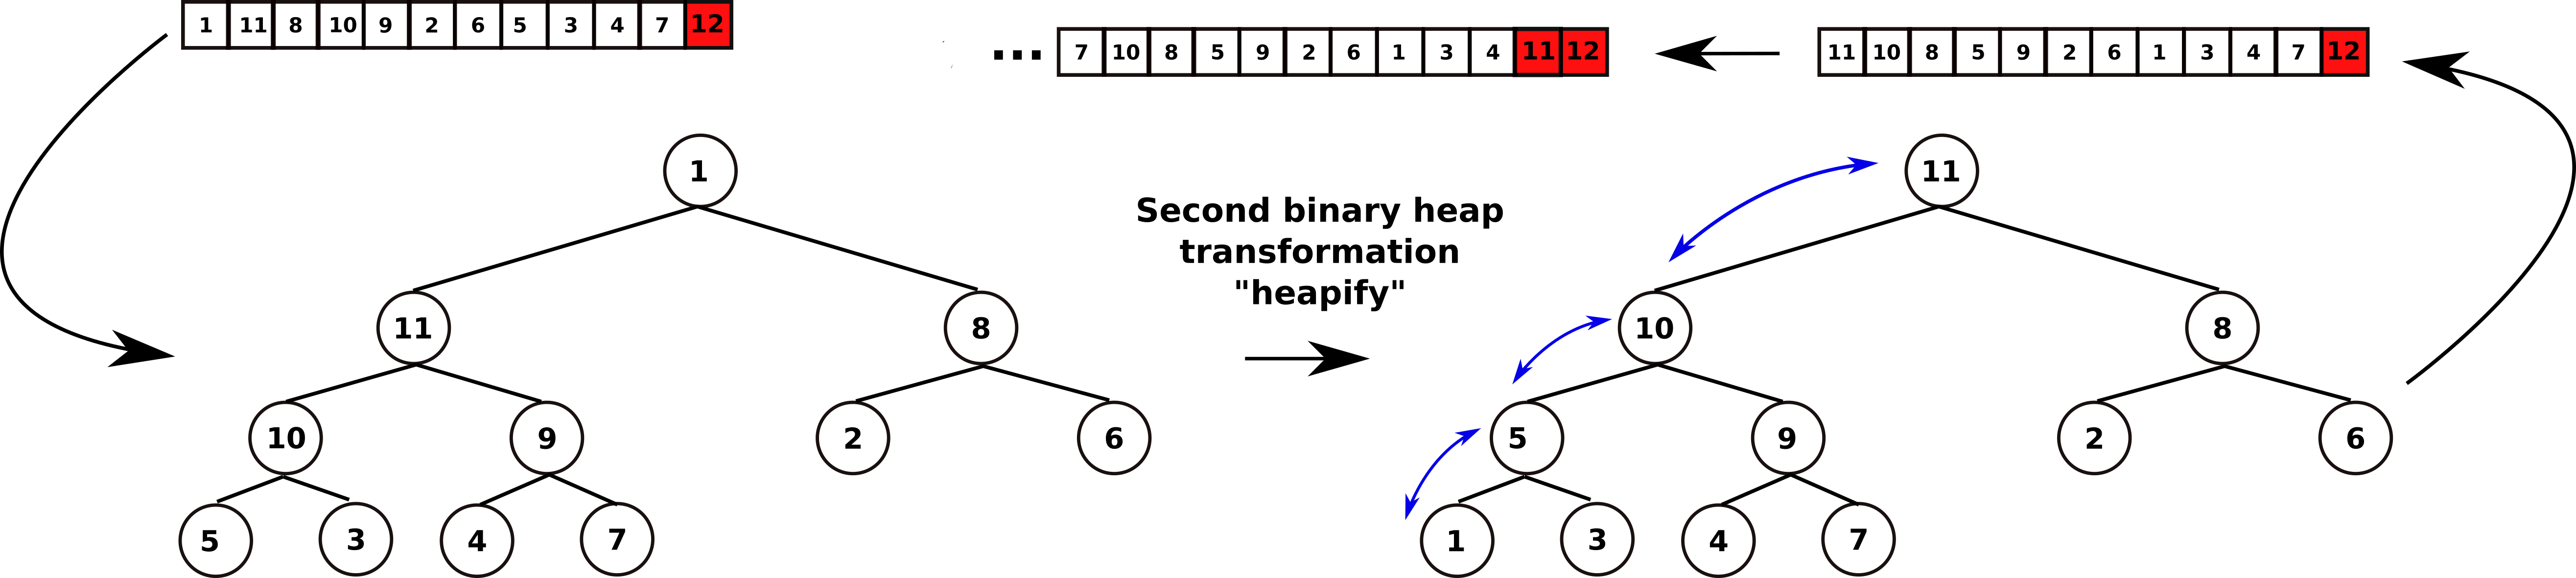
\includegraphics[scale=0.14]{images/heap_example_03.png} 
     	%\vspace*{-0.5em}
		%\caption{Floating gate transistor cell}
	\end{figure}	
	\end{center}	
	
	
	\end{frame}
	
	\subsection{Pseudo-code}	
	
	\begin{frame}
	
	\begin{columns}[c]
	\column{.8\textwidth} 
	\begin{center}    
    \scalebox{0.55} {
    %\begin{minipage}
    \begin{algorithm}[H]
    \SetAlgoLined   
	\SetKwProg{Fn}{Function}{ is}{end}
	\Fn{$build\_heap(Array)$} {
		i=$\frac{N}{2}$\;
		\While{i >= 1} {
			heapify(Array,i)\;	
			i=i-1\;	
		}	
	}
	
	\vspace*{1em}
	\Fn{$heapify(Array, i)$} {
		left=$2\times i$\;	
		right=$2\times i+1$\;
	
		\eIf{$(left <= N) and (Array[left] > A[i])$} {
			max=left\;
		} {
			max=i\;
		}	
		
		\If{$(right <=N) and (Array[right] > A[max])$} {
			max=right\;
		}		
		
		\If{$max != i$} {
			temp = Array[i]\;
			Array[i] = Array[max]\;
			Array[max] = temp\;
			$heapify(A, max)$\;		
		}	
	}
	  
    
    %\caption{Sequential search through the array}
	\end{algorithm}	
	%\end{minipage}
	}
	\end{center}			
	
	\column{.4\textwidth}
	\begin{flushleft}	
	\scalebox{0.55} {
	
	\begin{algorithm}[H] 

	//Heap-sorting code \\
	build\_heap(Array)\;
	i=N\;
	\While{i >= 1} {
		temp = A[1]\;
		A[1] = A[i]\;
		N=N-1\;
		$heapify(A, 1)$\;	
		j=j-1\;
	}	
	\end{algorithm}
	}
	\end{flushleft}	
		
	\end{columns}	
	
	\vspace*{2em}	
	
	Complexities: $O(N\times log(N))$	
	
	\end{frame}


	\section {Quick sort}
	\subsection{Principle}
	\begin{frame}
	
	\begin{block}{Principle}
	\begin{itemize}
	\item {Based on the \textbf{divide and conquer} approach}
	\item {Pick a \textbf{\textit{pivot}\footnotemark[2] element for partitioning} (first = last element)\footnotemark[3]}
	\item {For each \textit{pivot}: \textit{partitioning} = reordering the array: 
		\begin{itemize}
			\item {elements with \textbf{lesser values must be at the left of the pivot}}	
			\item {elements with \textbf{bigger values must be at the right of the pivot}}
			\item {we \textbf{change the position} of the pivot accordingly}
			\item {when \textbf{done = we change the pivot} \begin{enumerate}
				\item {new pivot = \textbf{element at the left of the previous pivot element}}
				\item {in this new partition\footnotemark[4], we rearrange elements as explained above}
				\item {we repeat (1) and (2) until reaching the extreme left}
				\item {we \textbf{do the same in the other direction} (new pivots will be on the right)}
			\end{enumerate}		
			}
		\end{itemize}			
	}
	\end{itemize}
	\end{block}	
	
	
	
	\footnotetext[2]{Pivot, like: \textit{pivoting}, or \textit{rotating} around something}
	\footnotetext[3]{Note that other approaches exist: taking the median element value, random, etc.}
	\footnotetext[4]{Partition: subpart of the array going from the pivot to the extreme left (or right)}	
	
	\begin{block}{Note}
	A practice: one of the fastest sorting algorithm
	\end{block}
	
		
	
	\end{frame}	
	

	
	
	\begin{frame}
	
	
	\begin{center}	
	\begin{figure}
		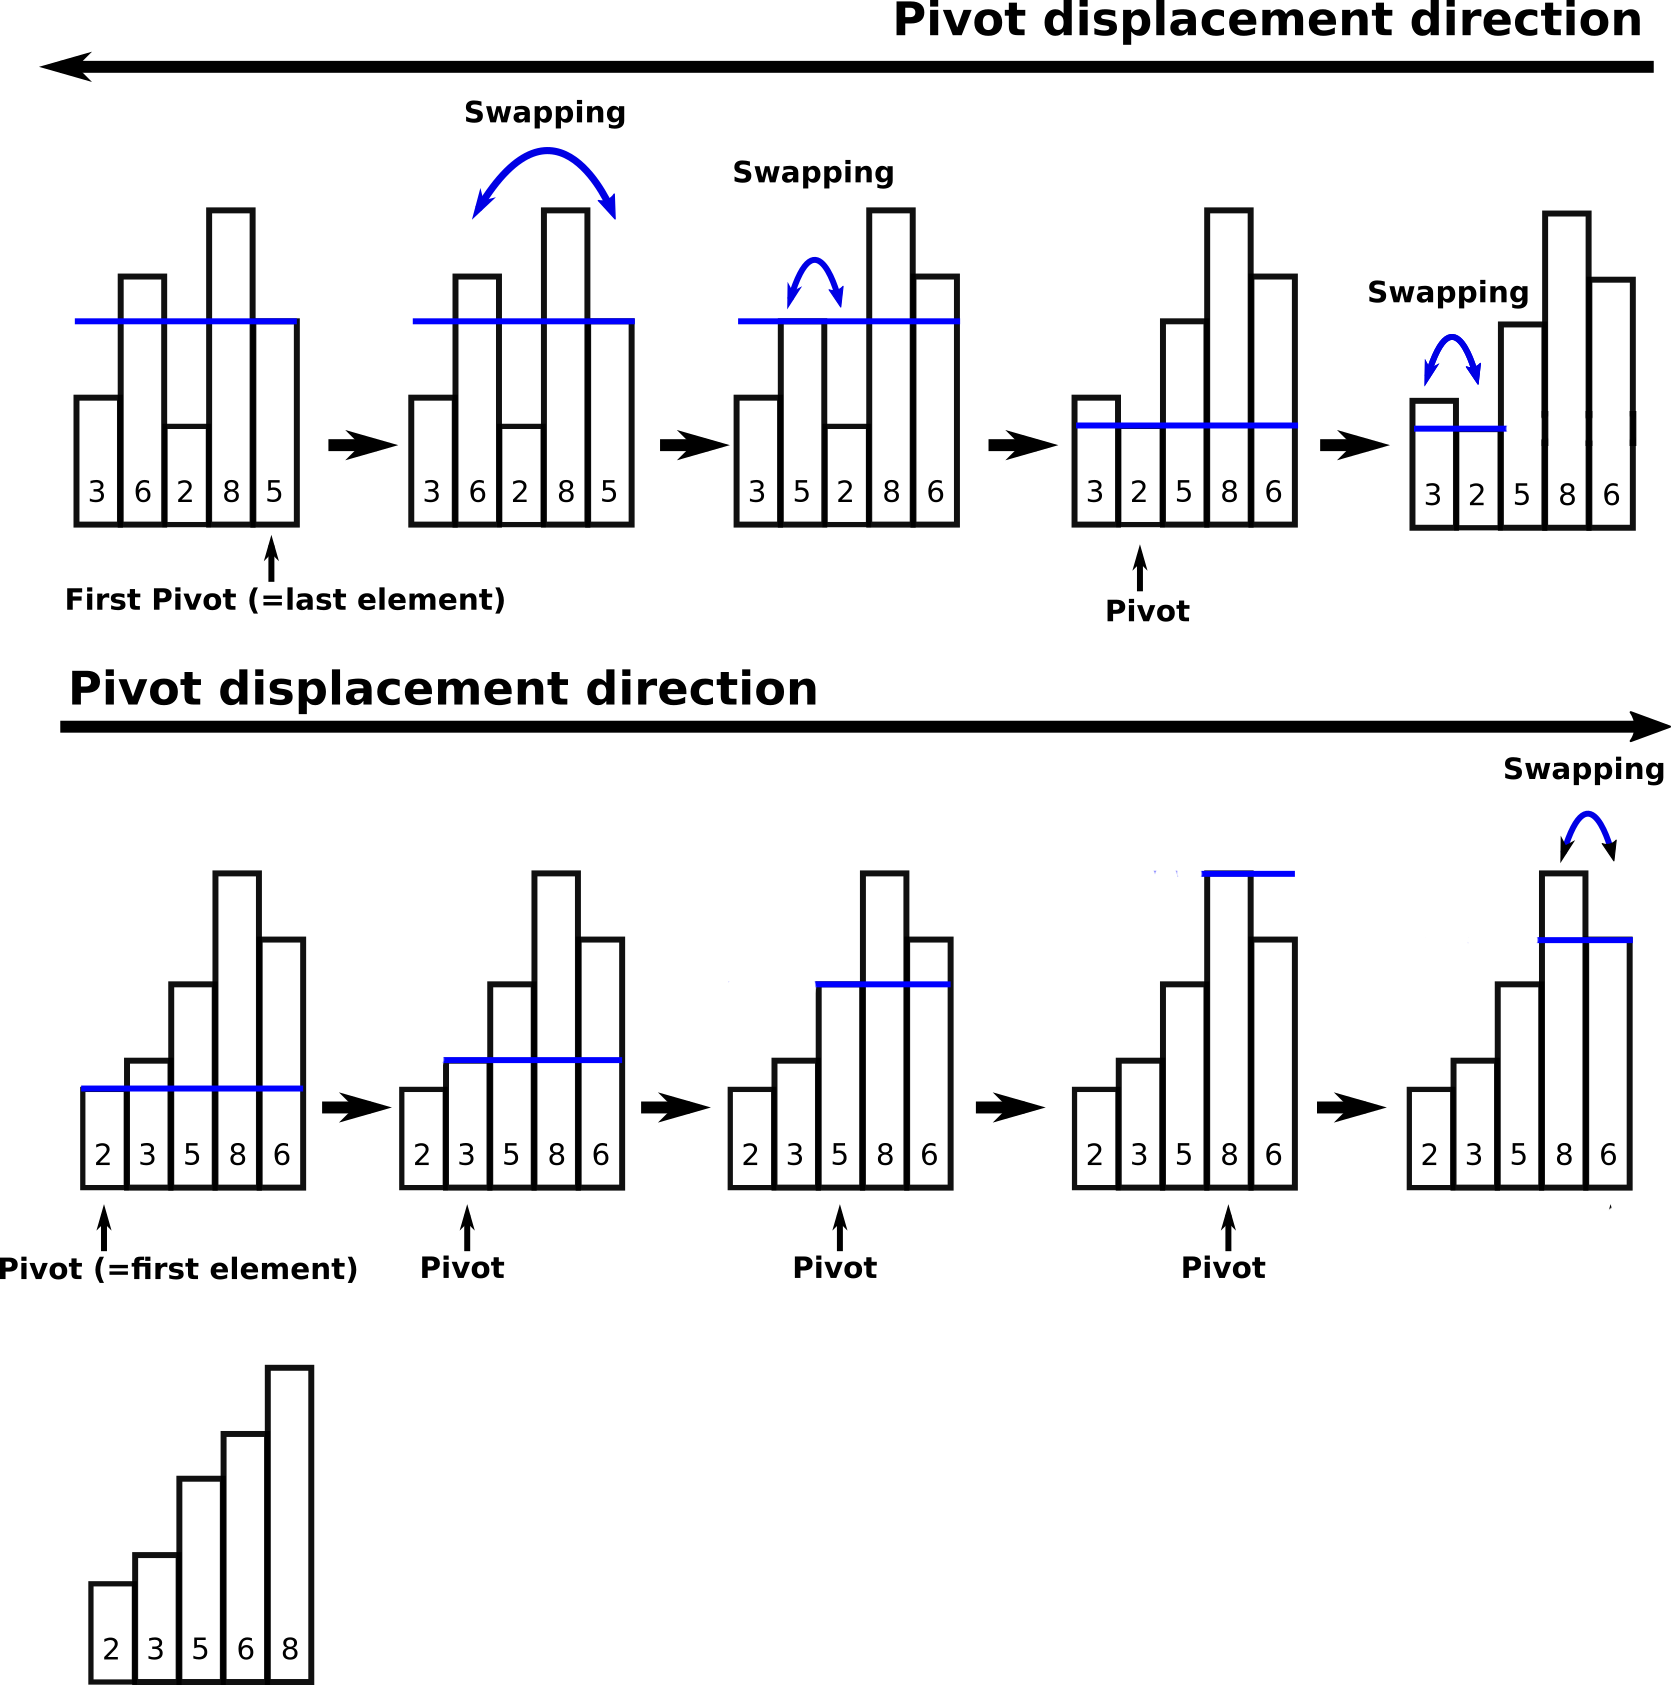
\includegraphics[scale=0.3]{images/quick_sort_01.png} 
     	%\vspace*{-0.5em}
		%\caption{Floating gate transistor cell}
	\end{figure}	
	\end{center}	
	
	
	\end{frame}
	
	

	\subsection{pseudo-code}

	\begin{frame}
	\begin{columns}[c]
	\column{.6\textwidth}
	\begin{center}    
    \scalebox{0.6} {
    %\begin{minipage}
    \begin{algorithm}[H]
    \SetAlgoLined   
	\SetKwProg{Fn}{Function}{ is}{end}
	\Fn{$partition(Array, low, high)$} {
		pivot=Array[high]\;
		i=low-1\;	
		j=low\;	
		\While{k <= high-1} {
			\If{Array[j] < pivot} {
				i=i+1\;
				temp=Array[i]\;
				Array[i]=Array[j]\;
				Array[j]=temp\;
			}
			temp=Array[i+1]\;
			Array[i+1]=Array[high]\;
			Array[high]=temp\;	
		}
		return i+1\;		
	}
    
    \vspace*{1em}
    \Fn{$quicksort(Array, low, high)$} {
    	\If{low < high} {
			p = partition(Array, low, high)\;
			quicksort(Array, low, p-1)\;
			quicksort(Array, p+1, high)\;	
		}	    
    }
        
    \vspace*{1em}
	//Quick sorting part \\
	quicksort(A, 0, N -1)\;    	
     	%\caption{InnserSequential search through the array}
	\end{algorithm}	
	%\end{minipage}
	}
	\end{center}
	\column{.55\textwidth}
	Complexities:
	\begin{center}
	\begin{itemize}
		\item {at best: $O(N\times log(N))$}
		\item {at worst: $O(N^2)$}
		\item {in average: $O(N\times log(N))$}
	\end{itemize}	
	\end{center}
	\end{columns}	
	
	\end{frame}

	

	\section{Summary}
	
	\begin{frame}
	
	\begin{itemize}
	\item {Selection sort: 
		\begin{itemize}
		\item {performs \textbf{few writes/swaps} in average (good for embedded systems)}
		\end{itemize}
	}
	\item {Selection and insertion sort: 
		\begin{itemize}
		\item {fast approach for \textbf{small arrays}}
		\end{itemize}
	}
	\item {Bubble: theoretically and in practice: \textbf{not a good solution}}
	\item {Heapsort: \begin{itemize}
		\item {best theoretical approach (\textbf{best time complexities})}
		\item {more suitable for \textbf{average to big arrays}}
		\end{itemize}
	}
	\item {Quicksort: \begin{itemize}
		\item {\textbf{not as good as heapsort theoretically}}
		\item {in practice: \textbf{fastest sorting approach}}
		\item {not fast if input array already sorted}
		\end{itemize}
		}		
	\end{itemize}
	
	\end{frame}	
	
	

\end{document}